\section{연구 결과}


\subsection{하드웨어 완성}
 제작한 모터포커서는 제어키와 숫자로 이루어져 있는 기호를 통해 통신을 한다. 예를 들어, a에 모터 시계방향 회전을 할당하고 a:100이라는 기호를 입력하면 모터는 시계방향으로 100step만큼 이동하게 되는 것이다. 보강한 모터포커서 또한 이러한 방법을 응용하였으며, 어떤 방법으로 제어에 성공하였는지 서술한다.
 
\subsubsection{열선 제어}

 앞서 설명하였듯 열선의 제어는 전압의 PWM을 이용하여 실행된다. \textrm{Figure} \ref{PWM}와 같이 시리얼 포트를 통한 입력을 할 때 필요한 기호는 A와 D이며, 0~100의 값을 입력받아 500ms 주기로 값을 변화시킬 수 있도록 설계하였다.
 
  \begin{figure}[ht]
 	\begin{center}
 		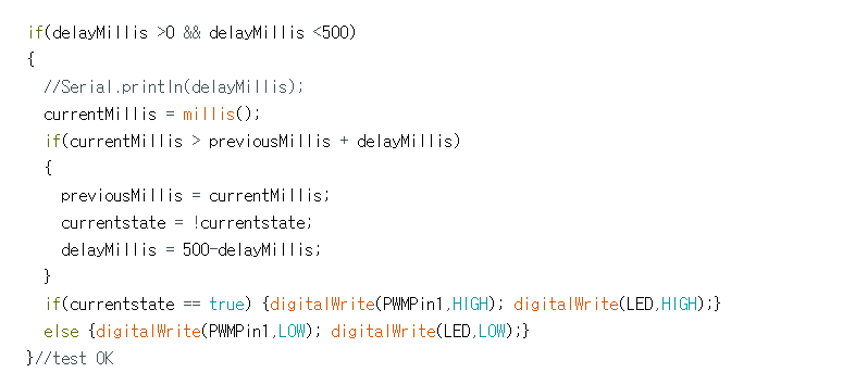
\includegraphics[width = 11cm]{PWMcode}
 	\end{center}
 	\caption{PWM제어를 위한 코드}
 	\label{PWM}
 \end{figure}
 
\subsubsection{EEPROM(Electrically Erasable Read-Only Memory)}

 \begin{figure}[ht]
	\begin{center}
		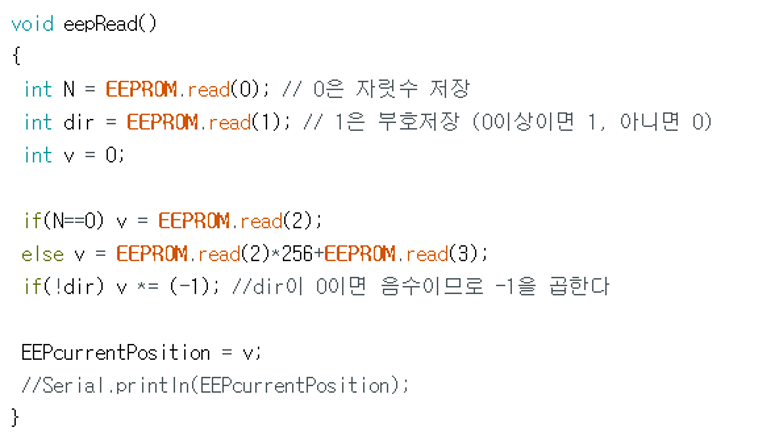
\includegraphics[width = 11cm]{eepread}
	\end{center}
	\caption{EEPROM에서 정보를 읽어오는 과정}
	\label{eepread}
\end{figure}

 모터포커서의 원활한 사용을 위해 저장되어야 하는 값은 모터의 위치를 저장할 수 있는 Position 값이다. \textrm{Figure}\ref{eepread}은 값을 EEPROM에서 읽어오는 과정을 나타낸 것으로, 모터포커서가 최초로 실행될 때 EEPROM에서 값을 불러오고, 모터를 움직여 값을 변화시킨 직후에 적용된 값을 EEPROM으로 입력시키면 EEPROM값과 모터포커서의 Position 값을 항상 동기화시킬 수 있다.
 
\subsubsection{서보모터 제어}
 일반적인 서보모터 또한 PWM을 응용하여 제어할 수 있으나, 대부분의 라이브러리에서 이미 그 값들을 적용시켜놓은 최적화 함수가 존재한다. 이를 활용하여 서보모터를 원하는 각도로 움직일 수 있도록 펌웨어 상에 코드를 제작하였다. 특히나 OLED를 활용하여 덮개에 부착된 마스크를 정확하게 제어할 수 있도록 하였다.
 
 시리얼 포트를 통한 입력을 할 때 필요한 기호는 N이며, 오직 0과 1만을 입력받아 각각의 상태로 서보모터를 제어한다.

	\begin{figure}[ht]
	\begin{center}
		\begin{tikzpicture}
		\node[anchor=south west,inner sep=0] at (0,0) 
		{
			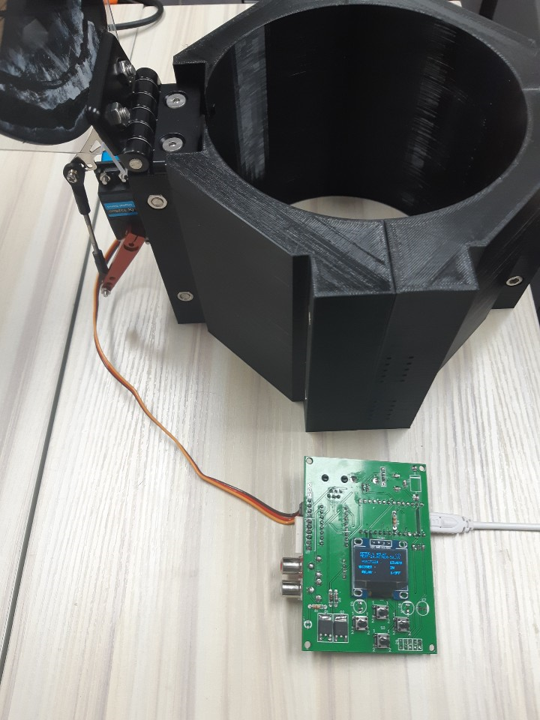
\includegraphics[height=7cm]{mask_status1}
			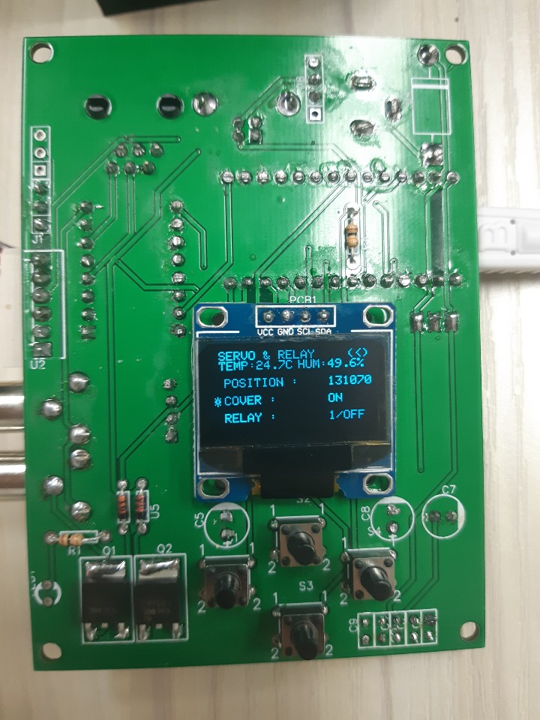
\includegraphics[height=7cm]{mask_status2} 
		};
		\draw (0.35, 0.3) node {(a)};
		\draw (5.7, 0.3) node {(b)};
		\end{tikzpicture}
	\end{center}
	\caption{(a) 개선된 모터포커서를 이용하여 제어한 덮개 (b) 이 때 개선된 모터포커서에 출력되는 마스크의 상태. 화면 아래의 버튼들을 이용해 상태를 제어할 수 있으며, 제어상태를 확인할 수 있다.}
\label{mask_status}


\end{figure}


 
\newpage
\subsection{ASCOM 드라이버}

 기존의 모터포커서의 여러 기능들이 추가됨에 따라, 기존에 만들었던 ASCOM 호환 드라이버 또한 업데이트를 할 필요성이 있었다. 때문에 여러가지 기능들을 추가하여 기존의 GUI를 발전시켰으며, Fig\ref{maincontrol}은 발전시킨 ASCOM 드라이버의 GUI의 모습을 나타내었다.
 
 \begin{figure}[h]
	\begin{center}
		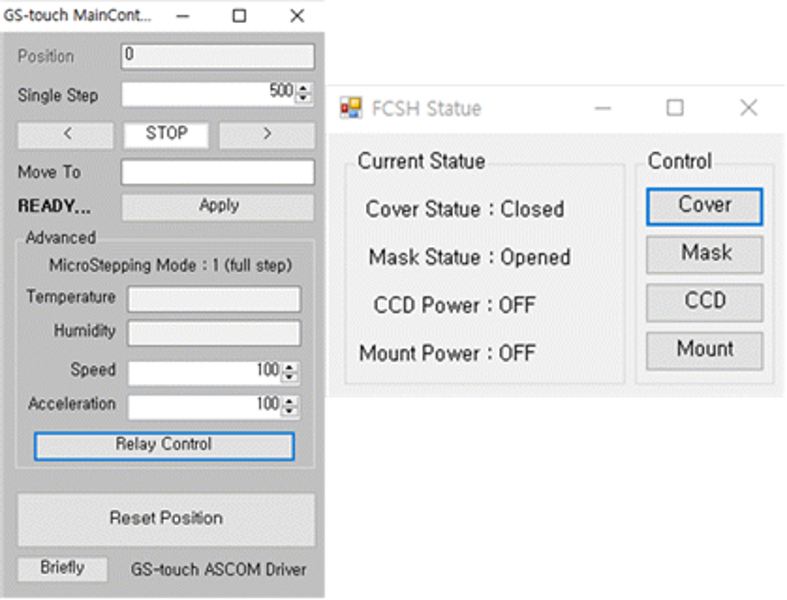
\includegraphics[width = 11cm]{maincontrol}
	\end{center}
	\caption{개선된 모터포커서 드라이버의 GUI 모습}
	\label{maincontrol}
\end{figure}

 기존의 모터포커서에서 추가된 기능인 덮개 제어기능, 열선 제어기능, Relay Control을 포함하고 있으며 각각의 Relay가 제어하는 기능들을 적었다.
